\documentclass[aspectratio=169,t,xcolor=table]{beamer}
\usepackage[utf8]{inputenc}

\usepackage{booktabs} 
\usepackage{subcaption}
\usepackage{epsfig}
\usepackage{siunitx}
\usepackage{physics}
\usepackage{setspace}
\usepackage{mathrsfs}
\usepackage{url}
\usepackage{lipsum}
\usepackage{animate}


\usetheme{UConn}

% ----------------------------------------------------------- Biblatex Citations
% \usepackage[
% backend=bibtex,
% style=ieee,
% ]{biblatex}
% \addbibresource{ECE5201_Citations.bib} %Imports bibliography file

% ------------------------------------------------------------- Bibtex Citations
% Optica Bibtex
\bibliographystyle{opticajnl}
\usepackage{jabbrv}
% \usepackage{footbib}

% \footbibliographystyle{opticajnl}
% \footbibliography{ECE5201_Citations}

% \usepackage{hanging}% http://ctan.org/pkg/hanging
% \setbeamertemplate{footnote}{%
%   \hangpara{2em}{1}%
%   \makebox[2em][l]{\insertfootnotemark}\footnotesize\insertfootnotetext\par%
% }

%-------------------------------------operators-------------
\newcommand{\dft}[2]{\frac{d^{#2}#1}{dt^{#2}}}
\DeclareMathOperator{\sinc}{sinc}
\DeclareMathOperator{\e}{e}
\DeclareMathOperator{\der}{d\hspace{-0.2em}}
\DeclareMathOperator{\proj}{proj}
\DeclareMathOperator{\sign}{sign}
\newcommand{\bX}[0]{\mathbf{X}}
\newcommand{\bv}[1]{\mathbf{#1}} 
\newcommand{\parallelsum}{\mathbin{\!/\mkern-5mu/\!}}
\newcommand{\vecc}[1]{\mathbf{#1}}

\newcommand\blfootnote[1]{%
  \begingroup
  \renewcommand\thefootnote{}\footnote[frame]{\tiny #1}%
  \addtocounter{footnote}{-1}%
  \endgroup
}

%-------------------------------------theorems--------------

\setbeamertemplate{theorems}[numbered]
\setbeamertemplate{caption}[numbered]

%-------------------------------------------------------------%
%----------------------- Primary Definitions -----------------%

% This command set the default Color, is also possible to 
% choose a custom color
\setPrimaryColor{UConnBlue} 

% First one is logo in title slide (we recommend use a
% horizontal image), and second one is the logo used in the
% remaining slides (we recommend use a square image)
\setLogos{lib/logos/UConnHusky.png}{lib/logos/UConnHusky.png} 


% -------------------------------------- Title Slide Information
\begin{document}
\title{Electromagnetics \& Anisotropy}
% \subtitle{Kevin Lindstrom}
\institute{Department of Electrical and Computer Engineering\\
 University of Connecticut}
\subtitle{Half-Waveplates, Quarter-Waveplates, and Uniaxial Media}

\author{Kevin Lindstrom\\
\textrm{\href{mailto:kevin.lindstrom@uconn.edu}{kevin.lindstrom@uconn.edu}}}
\date{April 27, 2023}


%-----------------------The next statement creates the title page.
\frame[noframenumbering]{\titlepage}


%------------------------------------------------Slide 1
\setLayout{vertical} % This command define the layout. 'vertical' 
% can be replace with 'horizontal', 'blank, 'mainpoint', 'titlepage'

\begin{frame}
    \frametitle{Table of Contents}\vspace{-1em}
    \begin{minipage}[t]{0.4\textwidth}
    \tableofcontents
    \end{minipage}
    \vline
    \hspace{1em}
    \begin{minipage}[t]{0.5\textwidth}
        % \centering
        % \animategraphics[loop,width=0.5\textwidth]{10}{HWP_aini_000}{0}{7}
        \begin{figure}[H]
            \centering
            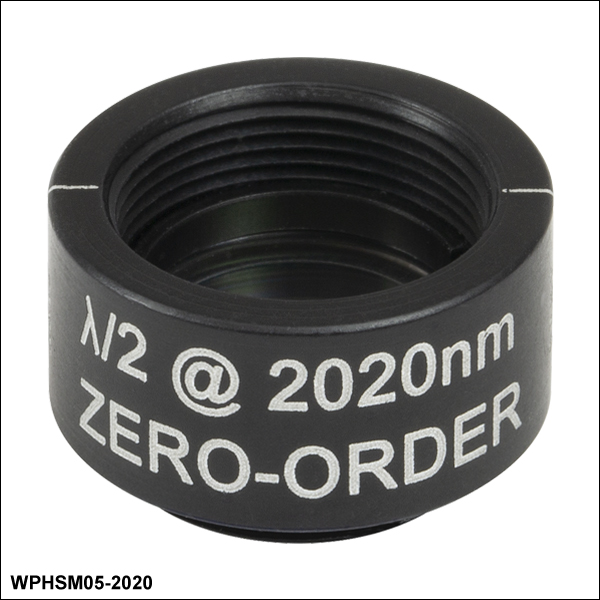
\includegraphics[width=0.63\textwidth]{figs/Waveplate.jpg}
            \caption{A picture of a half-waveplate (HWP) from Thorlabs \cite{WP}.
            HWPs rotate the polarization of LP light by $\ang{90}$ and 
            quarter-waveplates (QWP) convert LP light to CP and visa versa.}
        \end{figure}
    \end{minipage}
    \blfootnote{\tiny
        \cite{WP} Thorlabs, 
        \url{https://www.thorlabs.com/newgrouppage9.cfm?objectgroup_id=711}.
    }
\end{frame}
%-------------------------------------------------------------------------------
% BEGIN PRESENTATION
% ------------------------------------------------------------------------------

%------------------------------------------------------------------------ Theory
\section{Theory}
\subsection{The Displacement Field}
\begin{frame}
    \frametitle{The Displacement Field}
    The electric displacement field $\vecc{D}$ (with units 
    $\si{C\cdot m^{-2}}$) is defined as
    \begin{equation}\label{eq:D_deff}
        \vecc{D} = \epsilon_0 \vecc{E} + \vecc{P} 
        \color{red}
        = \epsilon \vecc{E}
        \color{black}
    \end{equation}
    where $\vecc{P}$ is the polarization of the material, and the \color{red} red
    \color{black} part of the equation is true given an isotropic dielectric
    \cite{griffithsEM}.\\
    \vspace{1em} \pause
    The 
    \color{orange} perpendicular \color{black} and
    \color{blue} parallel \color{black} 
    boundary conditions (BC) for the displacement 
    field on an interface are
    \begin{equation}\label{eq:D_BC}
        \color{orange}
        (\vecc{D}_2 - \vecc{D}_1)\cdot \bv{\hat{n}}_{12} = \sigma_f
        \color{black}\quad\text{and}\quad\color{blue}
        (\vecc{D}_2 - \vecc{D}_1) \times \bv{\hat{n}}_{12} =
       (\vecc{P}_2 - \vecc{P}_1) \times \bv{\hat{n}}_{12}
       \color{black} 
    \end{equation}
    where $\sigma_f$ is the free (unbounded) surface charge density, and 
    $\bv{\hat{n}}_{12}$
    is the normal vector of the interface from medium 1 to medium 2.
    \blfootnote{
        \cite{griffithsEM} D. J. Griffiths, \textit{Introduction to 
        Electrodynamics} (Pearson, 2013).
    }
\end{frame}

\subsection{Anisotropic Materials}
\begin{frame}
    \frametitle{The Displacement Field \& Anisotropy}\vspace{-1em}
    \begin{alertblock}{What is Anisotropy?}
        Materials are \textit{Anisotropic} if their properties have 
        \textbf{directional
        dependence}---permittivity could take
        two different values depending on if the $\bv{E}$ field is in the 
        $\bv{\hat{x}}$ or $\bv{\hat{y}}$ direction \cite{Balanis-2012}.
    \end{alertblock}\\
    \vspace{0.2em}\pause
    For anisotropic media, we use the relative permittivity tensor (rank 2), 
    which must be a Hermitian matrix \cite{CWA_S, Wav_anis}.
    \begin{equation}\label{eq:eps_ten}
        \bar{\epsilon}_r = \begin{bmatrix}
            \epsilon_{xx} & \epsilon_{xy} & \epsilon_{xz}\\
            \epsilon_{yx} & \epsilon_{yy} & \epsilon_{yz}\\
            \epsilon_{zx} & \epsilon_{zy} & \epsilon_{zz}\\
        \end{bmatrix}
        \quad\text{where}\quad
        \epsilon_{ij} = \epsilon_{ji}^*
    \end{equation}
    Equation \eqref{eq:D_deff} becomes
    \begin{equation}\label{eq:D_anis}
        \vecc{D} =  \epsilon_0\bar{\epsilon}_r \vecc{E}
    \end{equation}
    \blfootnote{
        \cite{Balanis-2012} C. A. Balanis, \textit{Antenna Theory: 
        Analysis and Design}
        (Wiley-Interscience, 2005).
    }
    \blfootnote{
        \cite{CWA_S} P. Beyersdorf, ``Coupled mode analysis,''
        % \url{https://www.sjsu.edu/faculty/beyersdorf/Archive/Phys208F07/ch\%204}.
        \url{https://www.sjsu.edu/faculty/beyersdorf/Archive/Phys208F07/ch\%204-EM\%20waves\%20in\%20anisotropic\%20media.pdf}.
    }
    \blfootnote{
        \cite{Wav_anis} F. Ran, ``Waves in Anisotropic Media,''
        \url{https://courses.cit.cornell.edu/ece303/Lectures/lecture17.pdf} (2007).
    }
\end{frame}

\subsection{Uniaxial Media}
\begin{frame}
    \frametitle{Uniaxial Media}
    Calcite, mica, and quartz are examples of \textit{uniaxial media}, where
    the permittivity tensor takes the form
    \begin{equation}\label{eq:PT_UA}
    \bar{\epsilon}_r = \begin{bmatrix}
        \epsilon^e_r & 0 & 0\\
        0 & \epsilon^o_r & 0\\
       0 & 0 & \epsilon^o_r\\
    \end{bmatrix}
\end{equation}\pause
Here, the $x$-axis is the \textit{extraordinary} axis, and $y$/$z$-axes 
are the \textit{ordinary} axes~\cite{Wav_anis}.\\
\vspace{1em}
\begin{block}{Wave Propagation}
    \begin{itemize}
        \item The permittivity has two values
        \item \textbf{Waves propagate at different speeds depending on their 
        polarization}
    \end{itemize}
\end{block}
\blfootnote{
        \cite{Wav_anis} F. Ran, ``Waves in Anisotropic Media,''
        \url{https://courses.cit.cornell.edu/ece303/Lectures/lecture17.pdf} (2007)
    }
\end{frame}

%------------------------------------------------------------------- Waveplates
\section{Analytical Design}
\subsection{Design Diagram}
\begin{frame}
    \frametitle{Half-Waveplate Diagram}\vspace{-1em}
    \begin{figure}[H]
        \centering
        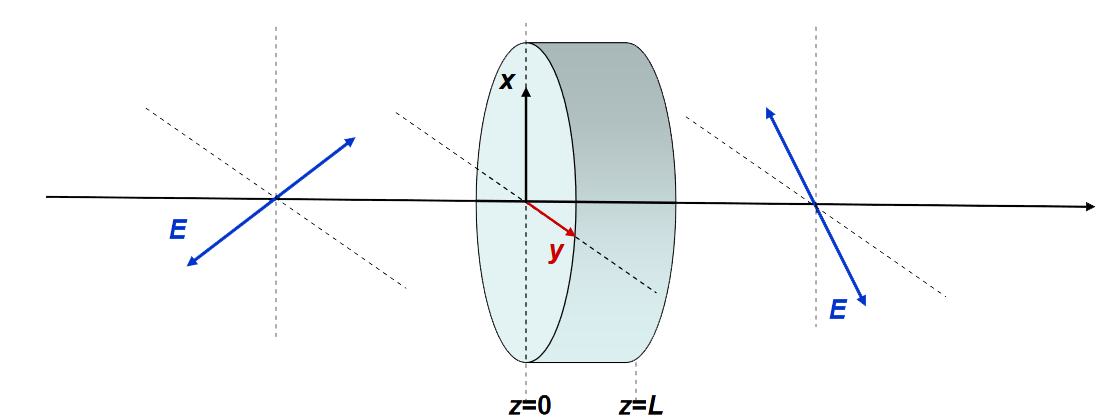
\includegraphics[width=\textwidth]{figs/HWP.PNG}
        \caption{
            A half-waveplate (HWP) in the $xy$-plane with length $L$ with an incident
            plane wave at $z=0$ \cite{Wav_anis}. HWPs rotate the polarization
            of an incident plane wave $\ang{90}$. We choose $z<0$ to be region 
            1, $0<z<L$ to be region 2, and $z>L$ to be region 3.
        }
        \label{fig:HWP}
    \end{figure}\vspace{-1em}
    \blfootnote{
        \cite{Wav_anis} F. Ran, ``Waves in Anisotropic Media,''
        \url{https://courses.cit.cornell.edu/ece303/Lectures/lecture17.pdf} (2007)
    }
\end{frame}

\subsection{Wave Equation}
\begin{frame}
    \frametitle{The Wave Equation}
    Using Faraday's Law, Ampere's Law, and Equation \eqref{eq:D_anis} we obtain
    the wave equation \cite{Balanis-2012, Wav_anis}
    \begin{equation}\label{eq:WaveEQ}
        \nabla \times \nabla \times \vecc{E}(\bv{r}) = 
        -j\omega \mu_0 \nabla \times \vecc{H}(\vecc{r}) = 
    \omega^2\mu_0 \vecc{D}(\vecc{r})
    \end{equation}
    which becomes
    \begin{equation}\label{eq:WaveEQ_simp}
        \nabla^2 \vecc{E}(\vecc{r}) =  -\omega^2\mu_0 \vecc{D}(\vecc{r})
        = -\omega^2\mu_0\epsilon_0 \bar{\epsilon}_r \vecc{E}(\vecc{r})
    \end{equation}\pause
    
    For normal incidence, a
    wave polarized in $\bv{\hat{x}}$ stays in $\bv{\hat{x}}$ in the dielectric
    \begin{equation}
        \vecc{E}^i_1(z) = \bv{\hat{x}}E_0 e^{-j\beta_0 z}
        \quad\Rightarrow\quad
        \vecc{E}^t_2(z) = \bv{\hat{x}}T_{12}^{e}E_0 e^{-j\beta^e z}
        % \left(\frac{2\sqrt{1/\epsilon^e}}{\sqrt{1/\epsilon_0} +
        %  \sqrt{1/\epsilon^e}}\right)
    \end{equation}\pause
    and $\bv{\hat{y}}$ stays in $\bv{\hat{y}}$
    \begin{equation}
    \vecc{E}^i_1(z) = \bv{\hat{y}}E_0 e^{-j\beta_0 z}
        \quad\Rightarrow\quad
        \vecc{E}^t_2(z) = \bv{\hat{y}}T_{12}^{o}E_0 e^{-j\beta^o z}
    \end{equation}
    \blfootnote{
        \cite{Balanis-2012} C. A. Balanis, 
        \textit{Antenna Theory: Analysis and Design}
        (Wiley-Interscience, 2005).
    }
    \blfootnote{
        \cite{Wav_anis} F. Ran, ``Waves in Anisotropic Media,''
        \url{https://courses.cit.cornell.edu/ece303/Lectures/lecture17.pdf} (2007)
    }
\end{frame}

\subsection{Half-Waveplate}
\begin{frame}
\frametitle{The Half-Waveplate}\vspace{-1em}
\begin{alertblock}{How do they work?}
    For just $\bv{\hat{x}}$ or $\bv{\hat{y}}$ incident polarization the 
    polarization inside the dielectric does 
    not change. How does a HWP cause the polarization to rotate?
\end{alertblock}\\\vspace{1em}\pause
Consider an incident wave \color{red}LP in $\bv{\hat{x}}$ and 
$\bv{\hat{y}}$\color{black}~\cite{Balanis-2012,Wav_anis}
\begin{equation}\label{eq:In_HWP}
    \vecc{E}^i_1(z) = 
    \left(\frac{\bv{\hat{x}} + \bv{\hat{y}}}{\sqrt{2}}\right)E_0 e^{-j\beta_0 z}
    \Rightarrow
    \vecc{E}^t_2(z) = 
    \frac{E_0}{\sqrt{2}}\left(
        \bv{\hat{x}}T_{12}^{e} e^{-j\beta^e z} +
        \bv{\hat{y}}T_{12}^{o} e^{-j\beta^o z}
    \right)
\end{equation}\pause
where (for a nonmagnetic material)
\begin{equation}
\beta^e = \omega\sqrt{\mu_0\epsilon^e_r\epsilon_0}
\quad\text{and}\quad
\beta^o = \omega\sqrt{\mu_0\epsilon^o_r\epsilon_0}
\end{equation}\pause
The field at $z=L$ becomes
\begin{equation}\label{eq:In_HWP_at_L}
    \left.\vecc{E}^t_2(z) \right|_{z = L}= 
    \frac{E_0}{\sqrt{2}}\left(
        \bv{\hat{x}}T_{12}^{e} e^{-j\beta^e L} +
        \bv{\hat{y}}T_{12}^{o} e^{-j\beta^o L}
    \right)
\end{equation}
\blfootnote{
    \cite{Balanis-2012} C. A. Balanis, \textit{Antenna Theory: 
    Analysis and Design}
    (Wiley-Interscience, 2005).
}
\blfootnote{
        \cite{Wav_anis} F. Ran, ``Waves in Anisotropic Media,''
        \url{https://courses.cit.cornell.edu/ece303/Lectures/lecture17.pdf} (2007)
    }
\end{frame}

\begin{frame}
    \frametitle{The Half-Waveplate Cont.} \vspace{-1.2em}
    For $\ang{90}$ polarization change we want to flip $\bv{\hat{x}}$ or 
    $\bv{\hat{y}}$, so we choose Equation~\eqref{eq:L_HWP}\footnote[frame]{\tiny
    $\mathbb{Z}$ is defined as the set of all integers.}    
    such that Equation~\eqref{eq:In_HWP_at_L}
    becomes Equation \eqref{eq:Func_HWP}~\cite{Balanis-2012,Wav_anis}.
    \begin{equation}\label{eq:L_HWP}
        L(\beta^e-\beta^o) = (2m+1)\pi
        \quad\text{where}\quad
        \forall m \in \mathbb{Z}
    \end{equation}\vspace{-0.7em}   \pause
    \begin{equation}\label{eq:Func_HWP}
        \begin{aligned}
        \left.\vecc{E}^t_2(z) \right|_{z = L} &
        = \frac{E_0}{\sqrt{2}}\left(
            \bv{\hat{x}}T_{12}^{e} e^{-j\left[\beta^oL + (2m+1)\pi\right]} +
            \bv{\hat{y}}T_{12}^{o} e^{-j\beta^o L}
        \right)\\
        & = \frac{E_0}{\sqrt{2}}e^{-j\beta^o L}\left(
            -\bv{\hat{x}}T_{12}^{e} + \bv{\hat{y}}T_{12}^{o} 
        \right)\\
        \end{aligned}
    \end{equation} \vspace{-1em}\pause
    \begin{block}{We have obtained the desired polarization change, with 
        limitations...}
        \begin{itemize}
            \item $\epsilon_r^e$ and $\epsilon_r^o$ are $\omega$ dependent
            \item The device must be a precise thickness $L$
        \end{itemize}
    \end{block}
    \blfootnote{
        \cite{Balanis-2012} C. A. Balanis, \textit{Antenna Theory: 
        Analysis and Design}
        (Wiley-Interscience, 2005).
    }
    \blfootnote{
        \cite{Wav_anis} F. Ran, ``Waves in Anisotropic Media,''
        \url{https://courses.cit.cornell.edu/ece303/Lectures/lecture17.pdf} (2007)
    }
    \end{frame}

    \subsection{Quarter-Waveplate}
    \begin{frame}
        \frametitle{The Quarter-Waveplate} \vspace{-1em}
        \begin{block}{}
            Quarter-waveplates (QWP) turn LP light into CP and visa versa, and
            we can use Figure \ref{fig:HWP} to design an achromatic QWP
        \end{block}\\\vspace{1em}\pause
         Using 
        \begin{equation}\label{eq:L_QWP}
            L(\beta^e-\beta^o) = (2m+1)\frac{\pi}{2}
            \quad\text{where}\quad
            \forall m \in \mathbb{Z}
        \end{equation}\pause
        Equation \eqref{eq:In_HWP_at_L} becomes 
        % \footnote[frame,1]{test}
        \begin{equation}\label{eq:Func_QWP}
            \begin{aligned}
            \left.\vecc{E}^t_2(z) \right|_{z = L} &
            = \frac{E_0}{\sqrt{2}}e^{-j\beta^oL}\left(
                \bv{\hat{x}}T_{12}^{e} e^{-j(2m+1)\pi/2} +
                \bv{\hat{y}}T_{12}^{o} 
            \right)\\
            & = \frac{E_0}{\sqrt{2}}e^{-j\beta^o L}\left(
                \mp j\bv{\hat{x}}T_{12}^{e} + \bv{\hat{y}}T_{12}^{o} 
            \right)\\
            \end{aligned}
        \end{equation} \pause
        Hence, if $T_{12}^e\approx T_{12}^o$\\
        \begin{center} 
            LP $\rightarrow$ CP \hspace{5em} \& \hspace{5em} CP $\rightarrow$ LP
        \end{center}
    
        \end{frame}


        \section{Numerical Design}
        \subsection{3D-Plots}
        \begin{frame}
            % \frametitle{Quartz HWP}
            \vspace{-0.7em}
            \begin{figure}[H]
                \centering
                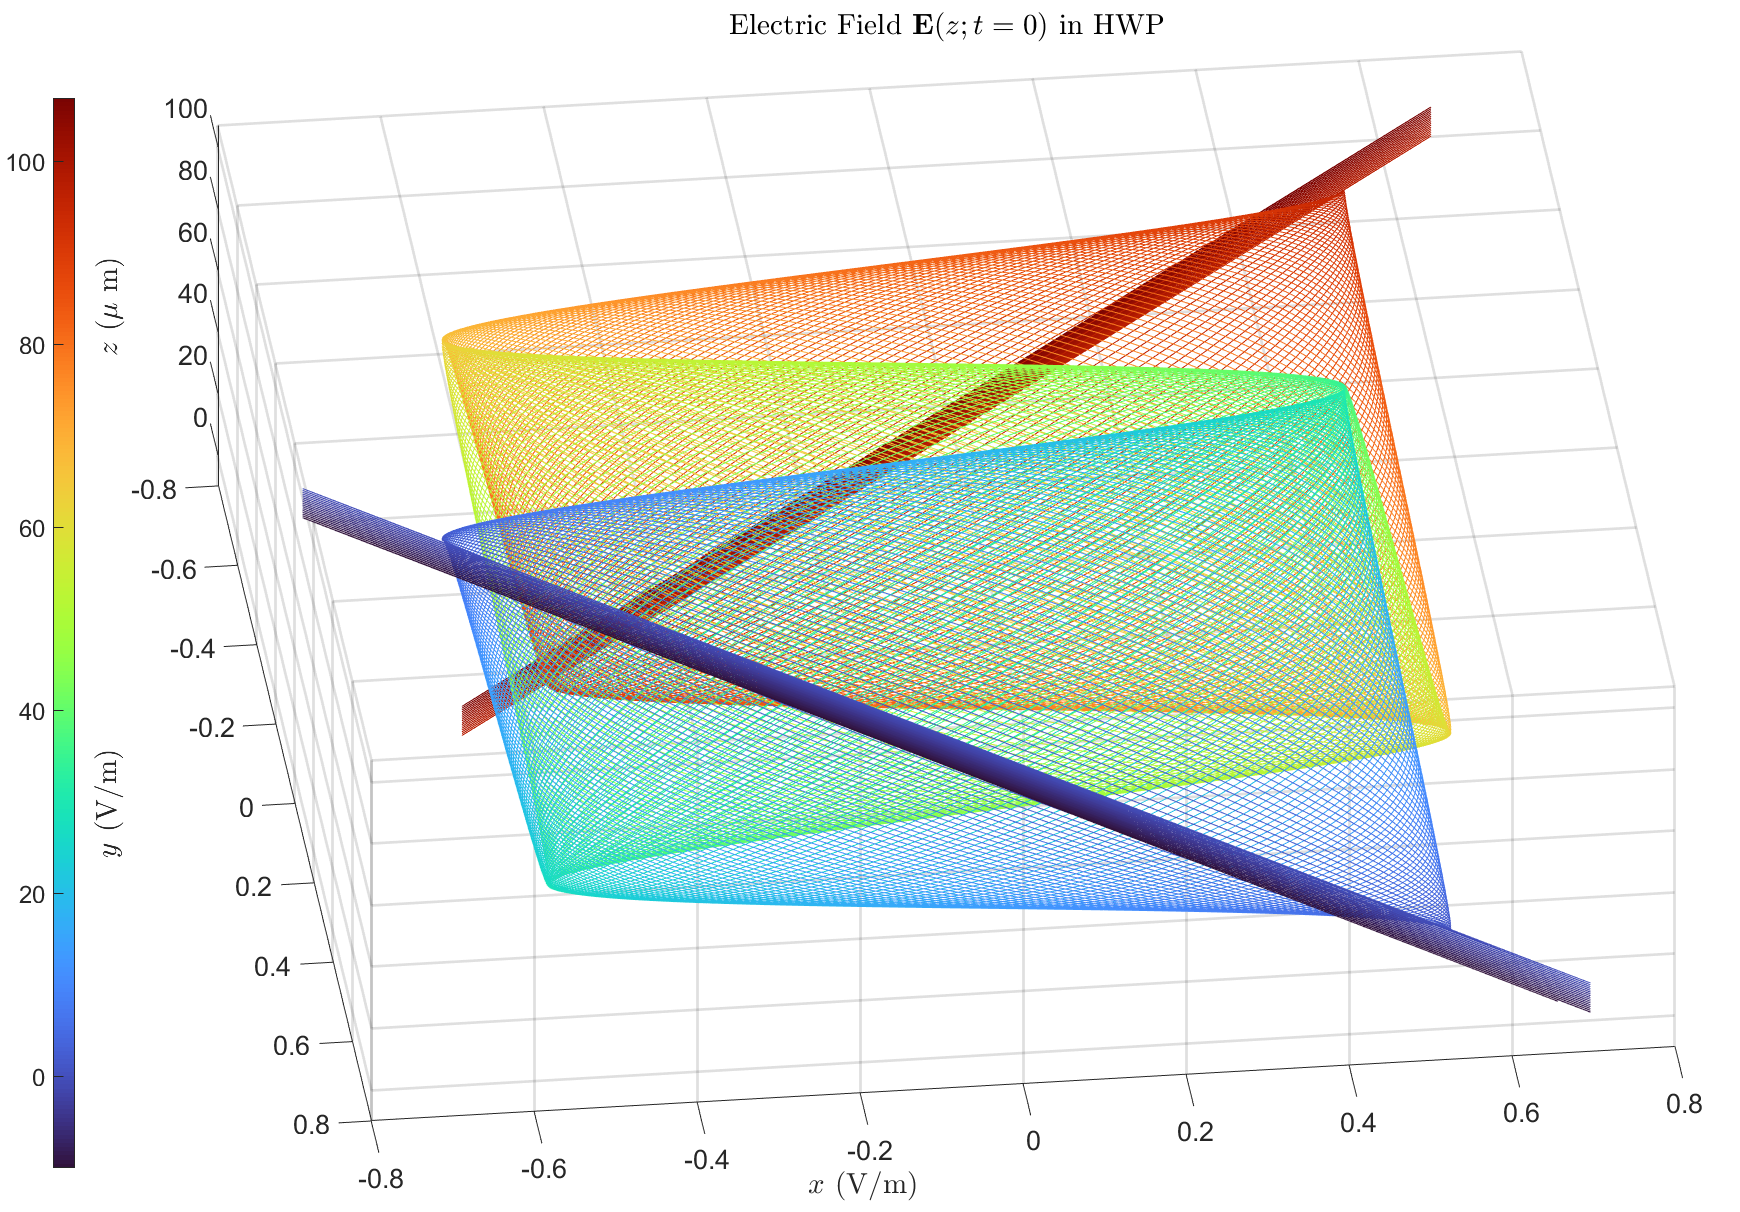
\includegraphics[width=0.82\textwidth]{figs/EfieldInHWP4.png}
                \vspace{-0.7em}
                \caption{
                    Forward propagating Electric Field before, inside, and after
                    a quartz HWP, $L = 96.933\si{\micro \meter}$ and 
                    $m=1$. Color bar helps visualize propagation in $z$.
                    Reflections not considered, discontinuities of 
                    $\vec{\mathscr{E}}(z; t= 0)$ would vanish they were.
                }
                \label{fig:Q_HWP}
            \end{figure}
        \end{frame}

        % \subsection{Quarter-Waveplate 3D-Plot}
        \begin{frame}
            % \frametitle{Quartz HWP}
            \vspace{-0.7em}
            \begin{figure}[H]
                \centering
                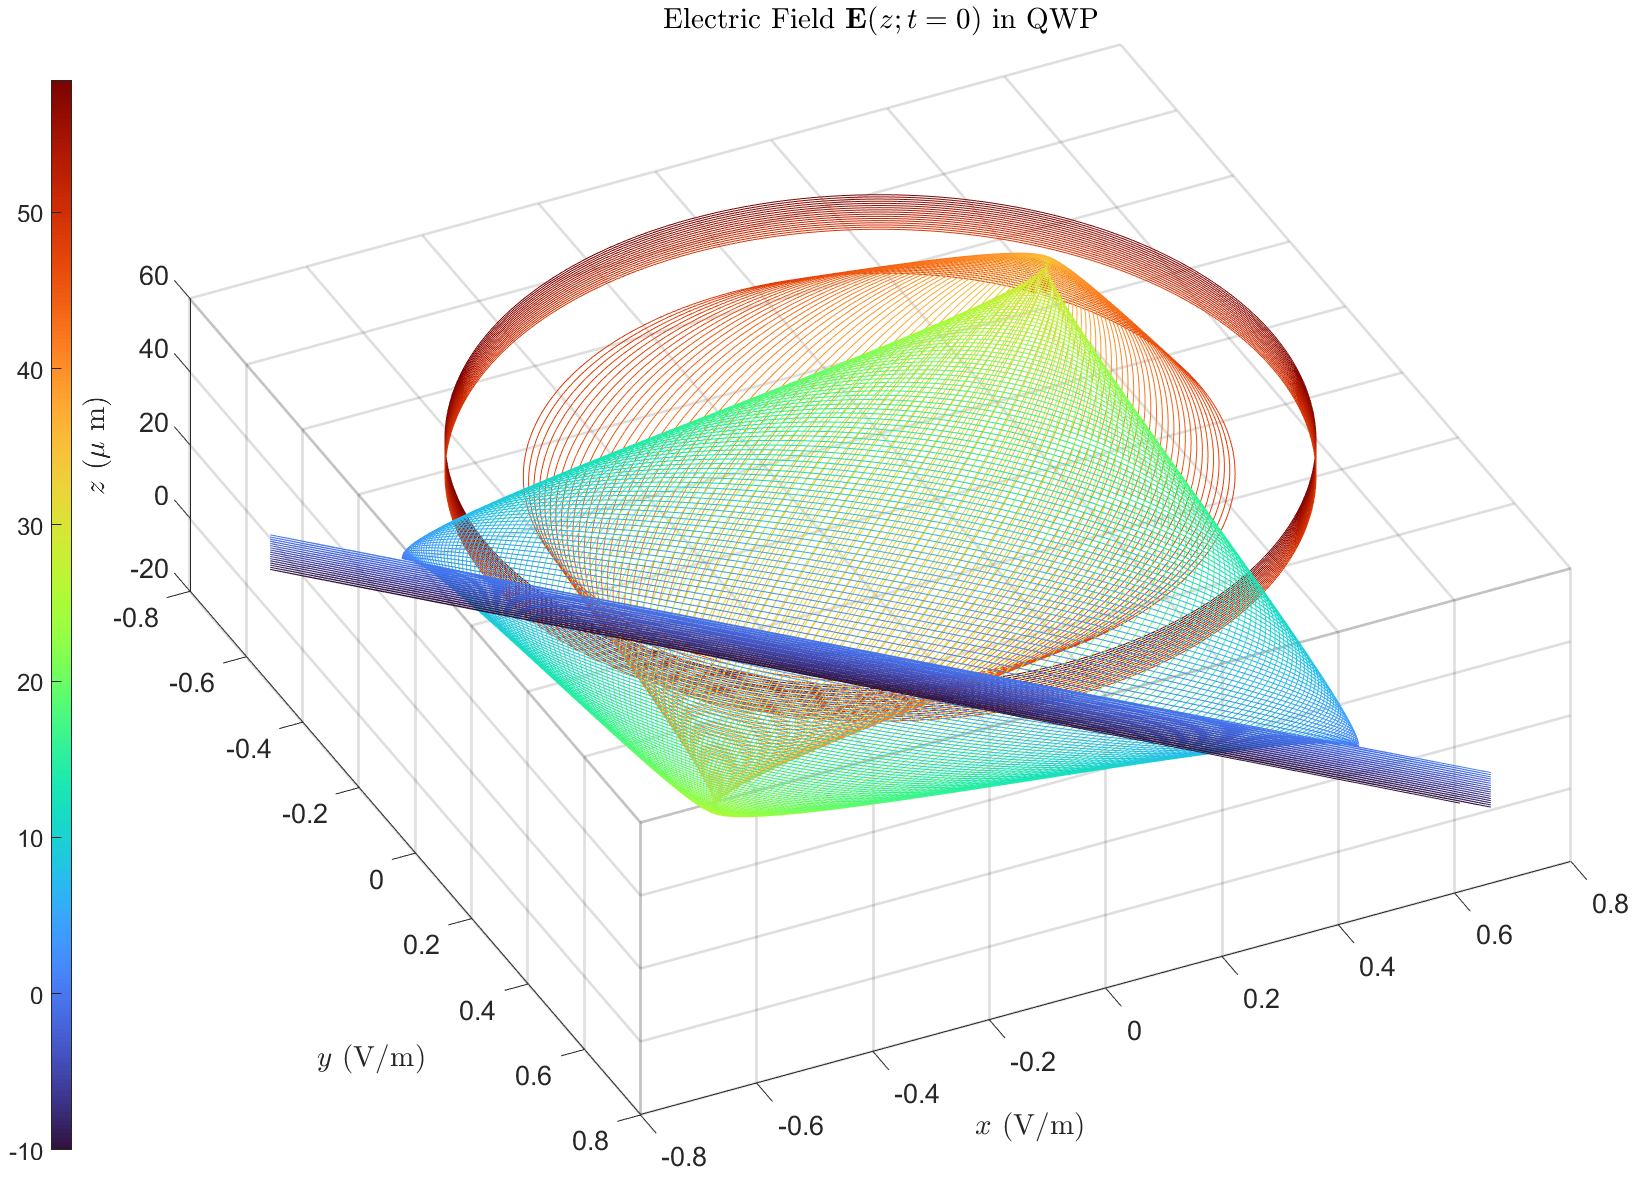
\includegraphics[width=0.8\textwidth]{figs/EfieldInQWP3.png}
                \vspace{-0.7em}
                \caption{
                    Forward propagating Electric Field before, inside, and after
                    a quartz QWP, $L = 48.4667\si{\micro \meter}$ and 
                    $m=1$. Color bar helps visualize propagation in $z$.
                    Reflections not considered, discontinuities of 
                    $\vec{\mathscr{E}}(z; t= 0)$ would vanish they were.
                }
                \label{fig:Q_QWP}
            \end{figure}
        \end{frame}

        % \begin{frame}{Limitatations}
        %     After the QWP
        %     \begin{equation}
        %         \bv{E}_3(z) = \frac{E_0}{\sqrt{2}}e^{-j\beta^o L}\left(
        %             \bv{\hat{x}}T_{23}^eT_{12}^{e}e^{-j(2m+1)\pi/2} + 
        %             \bv{\hat{y}}T_{23}^o T_{12}^{o} \right)e^{-j\beta(z-L)}
        %     \end{equation}
        %     When we evaluate these coefficients for our output field, we see
        %     it is slightly EP!
        %     $$
        %     T_{12}^oT_{23}^o - T_{12}^eT_{23}^e = 0.00121
        %     $$
        %     We also need to consider the round trip reflections of the device
        %     \begin{equation}\label{eq:ST_EF}
        %         \bv{E}_3(\bv{r}) = 
        %     \end{equation}
        % \end{frame}

        \begin{frame}
            \frametitle{Total Field after the Second Interface ($z>L$)}
            Half-wave plate:
              \begin{equation}\label{eq:E3_HWP}
                \bv{E}_3(z) = \xi(z)
                \sum_{n=0}^\infty e^{-j(2n+1)\beta^oL}
                \begin{bmatrix}
                    -T_{12}^e(\Gamma_{23}^e)^{2n}T_{23}^e\\
                    T_{12}^o(\Gamma_{23}^o)^{2n}T_{23}^o\\
                    0\\
                \end{bmatrix}
              \end{equation}
              Quarter-wave plate:
              \begin{equation}\label{eq:E3_QWP}
                \bv{E}_3(z) = \xi(z)
                \sum_{n=0}^\infty e^{-j(2n+1)\beta^oL}
                \begin{bmatrix}
                    -j(-1)^n(-1)^mT_{12}^e(\Gamma_{23}^e)^{2n}T_{23}^e\\
                    T_{12}^o(\Gamma_{23}^o)^{2n}T_{23}^o\\
                    0\\
                \end{bmatrix}
              \end{equation}
              where 
              $$
              \xi(z) \equiv \frac{E_0}{\sqrt{2}}e^{-j\beta_0(z-L)}
              \quad\text{and}\quad
              \forall m\in\mathbb{Z}
              $$
        \end{frame}

        \subsection{Figure of Merit}
        \begin{frame}
            \frametitle{Figures of Merit}\pause
            We define $R^\%$ as the ratio of the power of first internally 
            reflected and then transmitted wave $\bv{E}_3^{trrt}$ to the power 
            of the only forward propagating wave $\bv{E}_3^{tt}$
            \begin{equation}\label{eq:RP}
                R^\% = \frac{|\bv{E}_3^{trrt}|^2}{|\bv{E}_3^{tt}|^2} \cdot 100 = 
                \frac{
                \left[T^e_{12}(\Gamma^e_{23})^2T^e_{23}\right]^2 + 
                \left[T^o_{12}(\Gamma^o_{23})^2T^o_{23}\right]^2
                }{\left[T^e_{12}T^e_{23}\right]^2 + 
                \left[T^o_{12}T^o_{23}\right]^2} \cdot 100
                \end{equation}\pause
            We define the difference in the extraordinary and ordinary 
            transmission coefficients to be $\Delta T$
                \begin{equation}\label{eq:delta_T}
                    \Delta T = |T_{12}^e T_{23}^e - T_{12}^o T_{23}^o|
                  \end{equation}
            where ideally $\Delta T\approx 0$. 
        \end{frame}

        \subsection{Quartz Waveplates}
        \begin{frame}
            \frametitle{Designed Quartz Waveplates}
            For a quartz waveplate where $\epsilon_r^e=2.4130$ and 
            $\epsilon^o_r = 2.3847$ at $\lambda=590$ nm and non-magenetic 
            $\mu=\mu_0$ \cite{GHOSH199995}
            \begin{table}[h]
                \centering
                \begin{tabular}{ccccc}
                  Plate Type & $L$ ($\si{\micro m}$) & $m$ & $\Delta T$ & $R^\%$\\\hline \hline
                  HWP & 96.933 & 1 & 0.001 & 0.215\%\\\hline
                  HWP & 226.178 & 3 & 0.001 & 0.215\%\\\hline
                  QWP & 48.467 & 1 & 0.001 & 0.215\%\\\hline
                  QWP & 113.089 & 3 & 0.001 & 0.215\%\\\hline
                \end{tabular}
                \caption{Designed quantities and figures of merit.}
                \label{tb:Vals}
              \end{table}
              \blfootnote{\tiny
                \cite{GHOSH199995} 
                G. Ghosh, ``Dispersion-equation coefficients for the refractive 
                index and birefringence of calcite and quartz crystals,'' Opt. Commun.
                \textbf{163}, 95-102 (1999).
              }
        \end{frame}

        \subsection{Birefringence}
        \begin{frame}
            % \frametitle{Quartz HWP}
            \vspace{-0.7em}
            \begin{figure}[H]
                \centering
                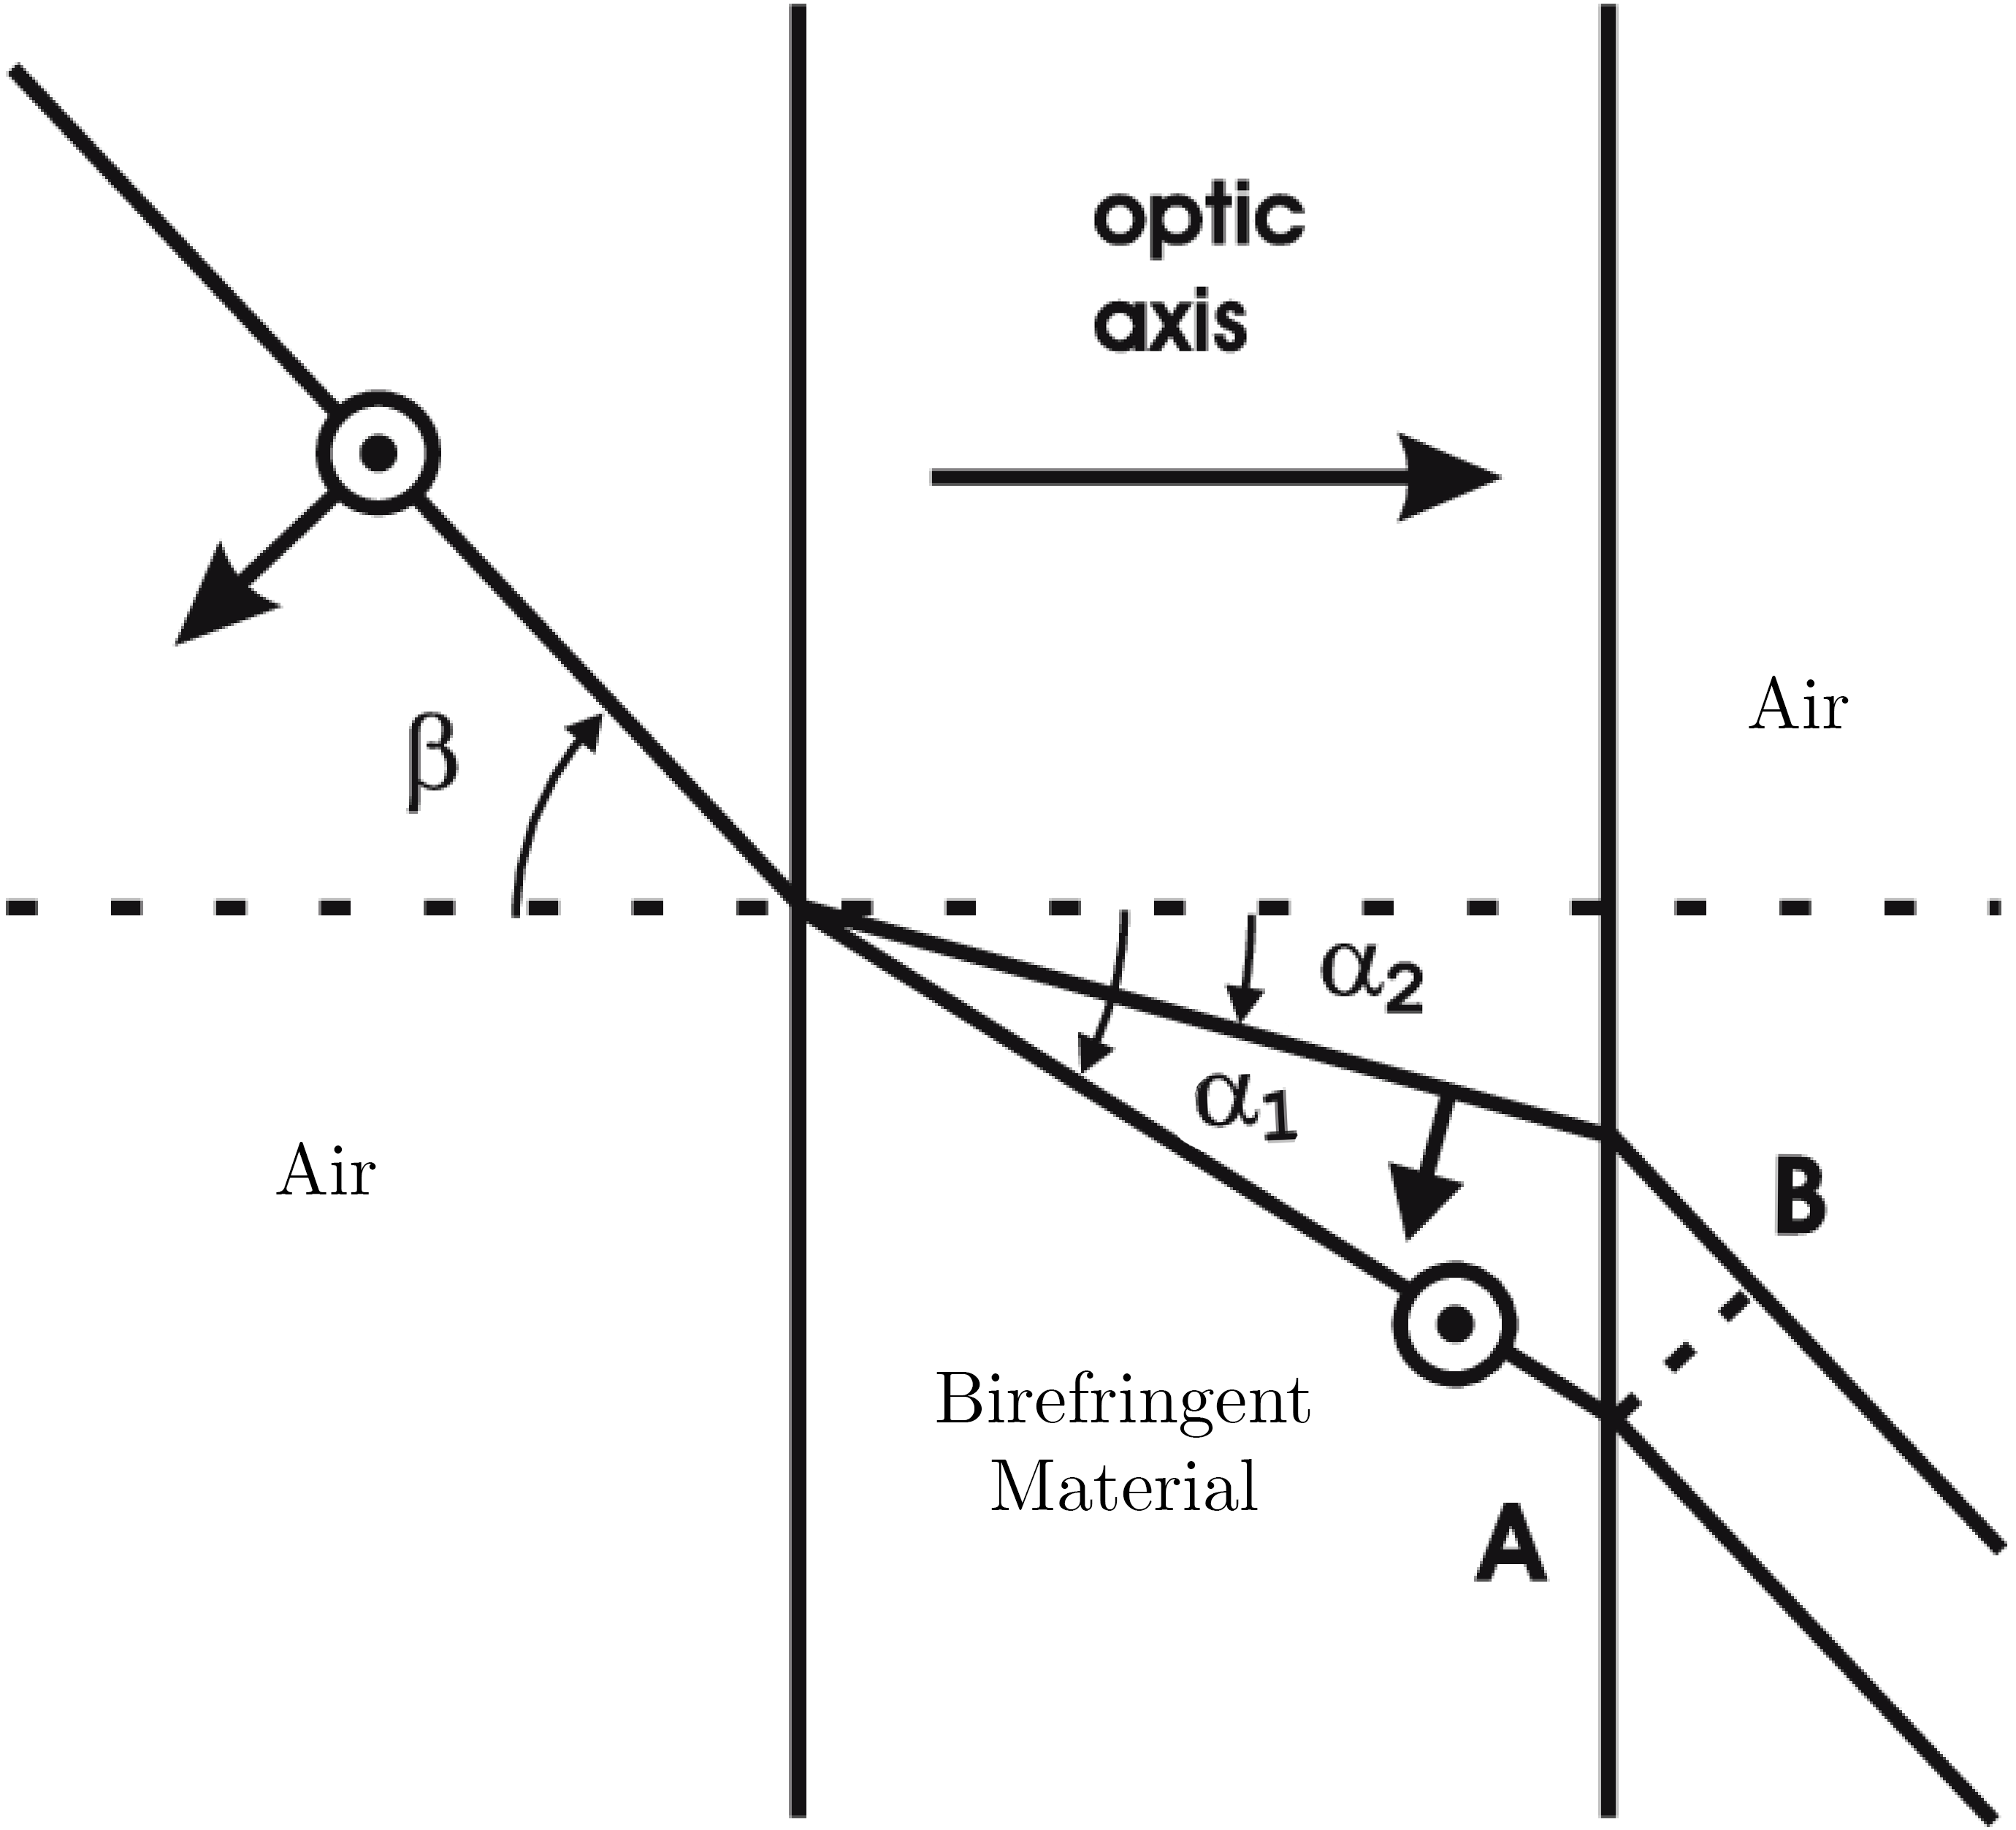
\includegraphics[width=0.6\textwidth]{figs/Birefringence.png}
                \vspace{-0.7em}
                \caption{
                    We obtain two spatially separated propagating fields when 
                    we consider
                    the case of oblique incidence on a \textbf{birefringent 
                    material} \cite{BR_IM}.
                }
                \label{fig:BR}
            \end{figure}\vspace{-2em}
            \blfootnote{
                \cite{BR_IM} A. Lutich, M. Danailov, s. Volchek, V. Yakovtseva, 
                V. Sokol, and S. Gaponenko, ``Birefringence of Nanoporous 
                Alumina: Dependence on
                Structure Parameters,'' Appl. Phys. B \textbf{84}, 327-331 (2006).
            }
        \end{frame}


\begin{frame}
    \frametitle{Citations}
    \vspace{-1.25em}
    \tiny
    % \printbibliography  % Biblatex
    \bibliography{ECE5201_Citations}  % Bibtex
    \vspace{1em}
    \begin{minipage}[t]{0.6\textwidth}
        \vspace{-6em}
        
        \textbf{Funding:}
        This research is unfunded.\vspace{0.7em}\noindent\\
        \vspace{0.7em}\noindent
        \textbf{Acknowledgments:}
        The author thanks T. Saule
        for his helpful conversations.\\
        \vspace{0.7em}\noindent
        \textbf{Disclosures:}
        The authors declare no conflicts of interest.\\
        % \vspace{0.5em}\noindent
        \textbf{Data Availability:} \LaTeX and MATLAB code for this project and
        its reports can be found on the author's github:\\
        \url{https://github.com/kevinlindstrom/ECE5201_TermProject}.
    \end{minipage}
    \begin{minipage}{0.35\textwidth}
        \begin{figure}[H]
            \centering
            
\includegraphics[width=0.65\textwidth]{figs/Github.png}
        \end{figure}
    \end{minipage}
   
\end{frame}


\setLayout{mainpoint}
%\setBGColor{UConnLightBlue}
\begin{frame}
    \frametitle{Questions?}
\end{frame}

\end{document}